\section{Lexer and parser generation}

%what the lexer and parser is
%differences
%how it is used
%why it is used
%how we generate them
%alternatives
This section will briefly cover how the lexer and parser for Arc has been implemented, and what alternatives could have been used.

For Arc, \gls{antlr} has been used, for creating the grammer and also to generate both the lexer and parser. From writing the grammar, is was possible for \gls{antlr} to generate the lexer, parser and more.\cite{Parr2014} This made \gls{antlr} highly effective for designing Arc, as small changes to the grammar could easily be made, without having to re-create the lexer and parser everytime. Instead only the grammar had to be changed, and \gls{antlr} would generate a new lexer and parser, based on the new grammar.

The grammar was made in a file called 'arcv2.g4' which is an \gls{antlr} file, that \gls{antlr} recognizes and also the lexical rule were made in a file called 'lexerRules.g4'. With these files, \gls{antlr} could generate all needed files for the parser, the lexical analyzer, and other supporting files. These files can be seen in the image \ref{fig:lexerandparserfiles}

\begin{figure}[htb!]
    \begin{center}
        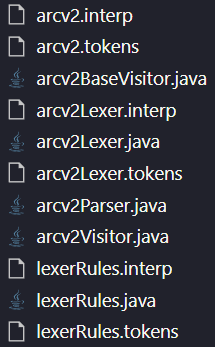
\includegraphics{figures/lexerAndParserFiles.png}
        \caption{Files generated for Arcs parser and lexical analyzer}
        \label{fig:lexerandparserfiles}
    \end{center}
\end{figure}

Figure \ref{fig:lexerandparserfiles} shows all files that \gls{antlr} generates, from the grammar rules and lexical rules. The file 'arcv2Parser.java' is the parser.\todo[]{Describe how the parser works and how it is used. Show code example!}


Another option to this could have been by writing out both the parser and lexer by hand, this could be very educational, as creating our own parser and lexer, would give in-depth knowledge of how they each work. But this would increase the time needed to create Arc considerably as, as mentioned previously, any minor change made in the grammar, would also mean going through the lexer and parser to fix them accordingly. This could lead to time wasted, which is a limiting factor for this project. Therefore it was decided to use the obviouse solution, to use the tools that readily avaliable. For this reason in particular, using \gls{antlr} to generate the lexer and parser for us, was the obviouse choice. 



\todo[inline]{Consinder adding examples of how we specifically have done it and discuss the files generated}

%The lexer, also called a lexical analyzer or scanner, takes a character stream and turns it into tokens. Tokens are a representation of something in a language, such as a num in Arc would be a token, that represents numbers. The lexer recognizes and can discard tokens of the character stream, so that the parser can ignore them. This includes tokens such as comments and whitespaces, that the parser does not need to concern itself with. If the lexer did not discard these tokens, that parser would constantly have to check for them. These tokens are then passed to the parser, that makes syntatic sense of them. It compares the tokens and their structure to the grammar of the specific language.\cite{Parr2014}


